This paragraph will present the two dashboards implemented, the design principles used, and the SA demons that were tried to avoid. As mentioned before, to ensure that most of the requirements identified in the previous stage could be represented, it was decided to use a dataset entirely created by us to have full control over the data and its structure.

The whole system is divided into two dashboards, each associated with multiple goals. The first dashboard aims to estabilish \textbf{Common Operational Picutre} that allows students to have a shared understanding of the current situation by integrating multiple subgoals into coherent visualizations. 
In contrast, the second dashboard, focuses on tracking and presenting student learning progress within a specific course.

\begin{itemize}
    \item \textbf{Dashboard I}: Subgoal 1.2.1 - Improve student engagement with the platform and Subgoal 1.2.2 - Optimize student learning through personalization.
    \item \textbf{Dashboard II}: Subgoal 1.1.1 - Comprehension of the fundamental concepts of cybersecurity and Subgoal 1.2.1 - Improve student engagement with the platform and Subgoal 1.2.2 - Optimize student learning through personalization.
\end{itemize} 

Both of the dashboards attempt to achieve the trade-off between supporting the operator's goal and supporting the overall SA. By placing the most important information appropriately at the center of each dashboard and positioning the supporting information on the sides, we ensure that critical data is easily accessible while still providing a comprehensive view. 

Additionally, the dashboards are designed to be user-friendly, with a clean and intuitive interface that allows students to quickly understand the information presented. This design choice is intended to reduce the cognitive load on the student, making it easier to process the data and make informed decisions, thereby further supporting individual objectives and improving situation awareness.

To limit complexity, and effort has been made to always provide explicit support SA Level 2, where necessary, so that information about his learning progress is always available to the student. In this way, the student can quickly understand his current situation and make informed decisions about his learning path.



\section{Dashboard I: Improve student engagement with the platform and optimize student learning through personalization}

The subgoals of this dashboard are to not lose the student's engagement with 
the platform and to help in adapting the learning process to the student's
needs. 

To make the student aware that he/she is looking
at the home page of the platform the name \textit{OffSec} is added,
which states for \textit{Offensive Cybersecurity}, that is the field
in which the student has to upskill his/her expertise. To remark that this
dashboard is the home page is added \textit{Welcome Marta!} message.
These two elements help the student to not use the wrong mental model
when he/she has to interpret the elements present inside the dashboard.
In this way, the \textbf{Wrong Mental Model} demon is avoided.

\begin{figure}[H]
    \centering
    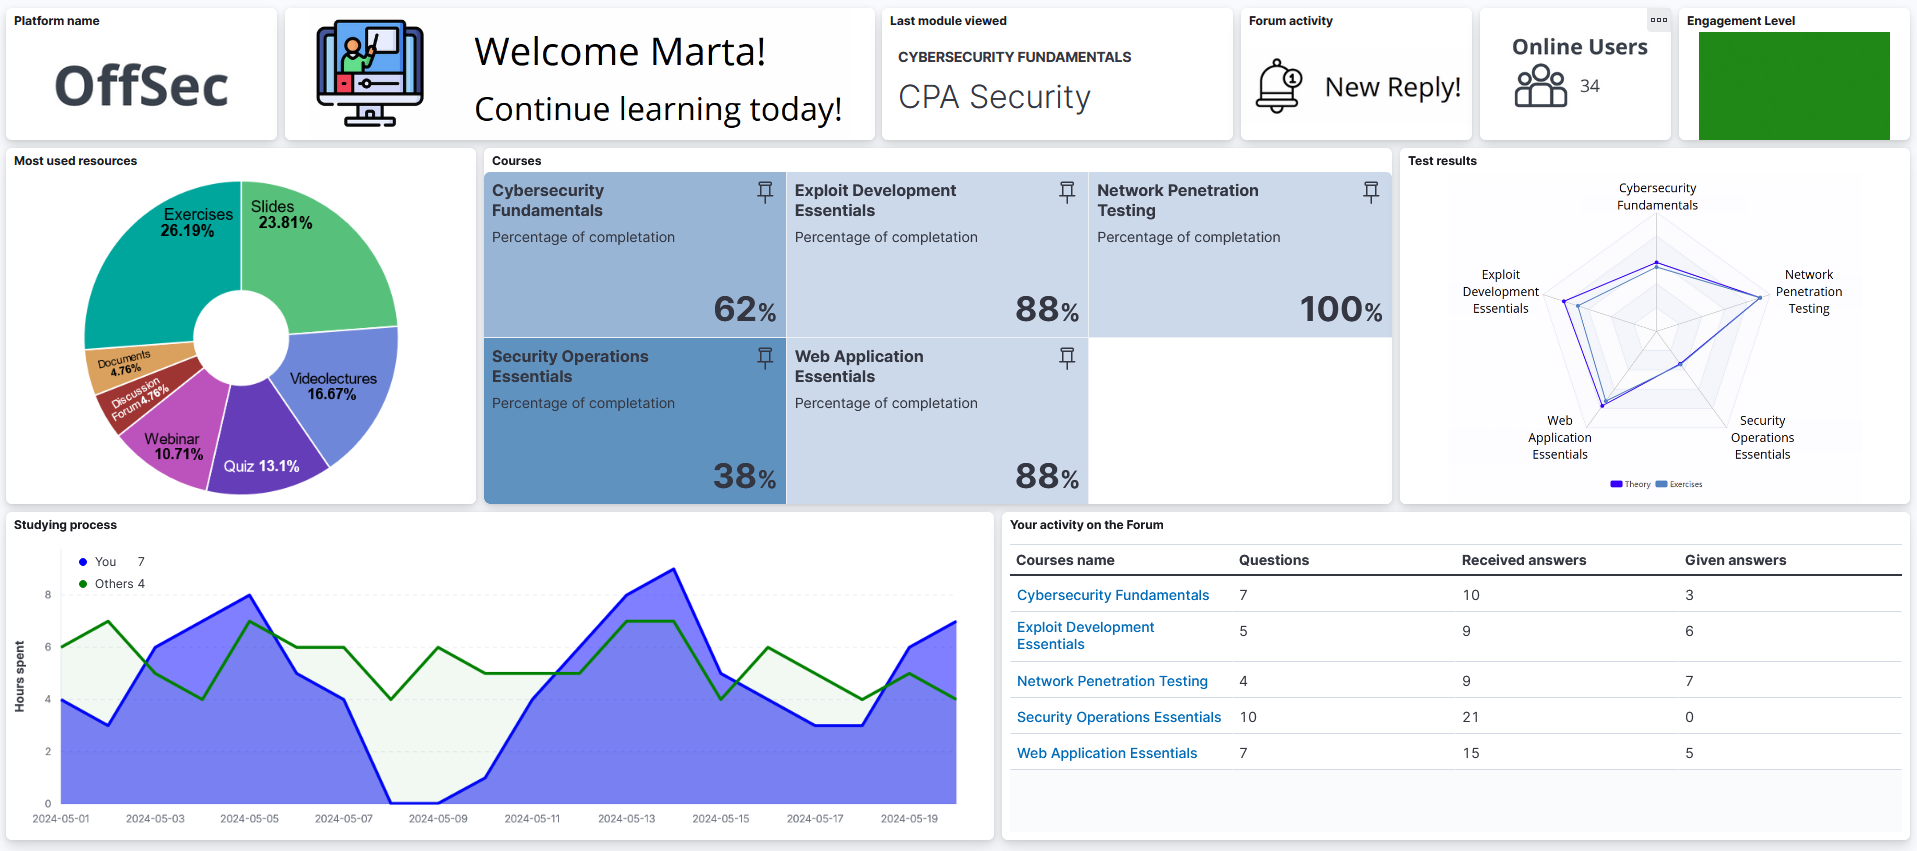
\includegraphics[width=0.9\textwidth]{assets/dashboard_1.png}
    \caption{Dashboard I}
    \label{fig:dashboard_1}
\end{figure}

Now is analyzed the different parts of the dashboard, discovering which
elements allow to achieve the goal of the student and which of them guarantee the
global situation of the student. The \textbf{subgoal 1.2.1} is guaranteed by the linear graph,
which shows the student's time spent on the platform since the start of
the process of upskilling. Also, this subgoal is guaranteed by the table containing the activity of the
student on the forum, showing how many questions the student asked, how many
answers received and how many answers the student has given. 
Both the elements are shown in the following figure.

\begin{figure}[H]
    \centering
    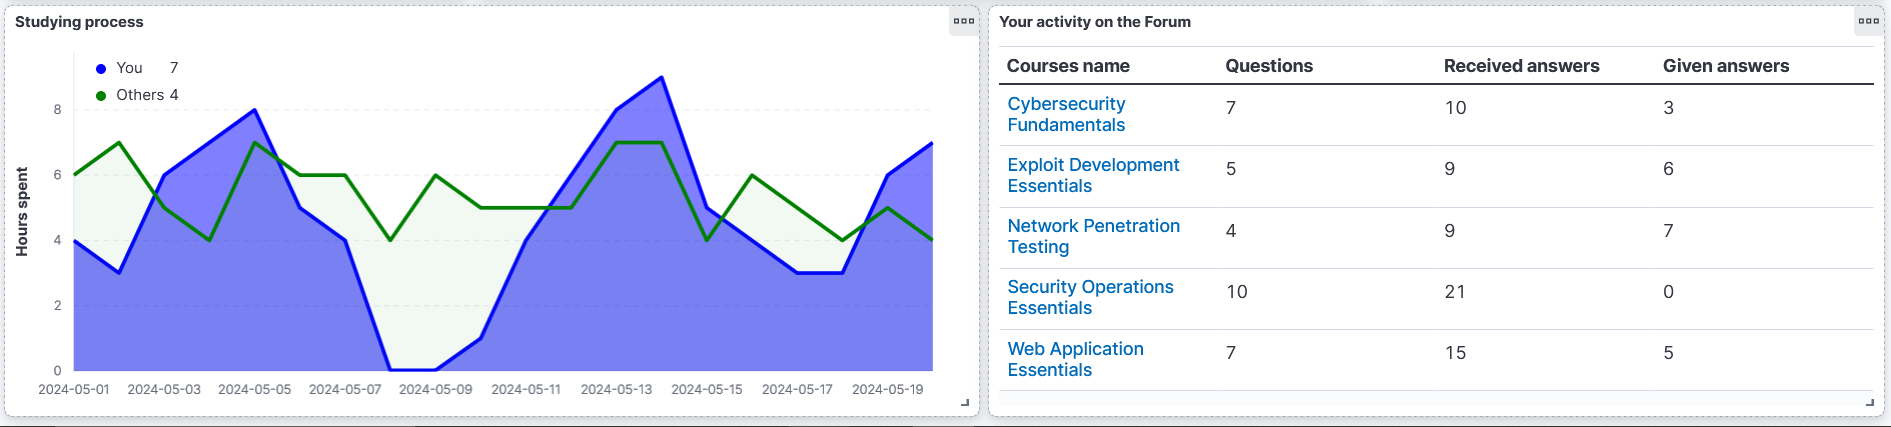
\includegraphics[width=0.9\textwidth]{assets/dashboard_1_121.png}
    \caption{Dashboard I - Subgoal 1.2.1}
    \label{fig:dashboard_1_subgoal_121}
\end{figure}


The \textbf{subgoal 1.2.2} is guaranteed by the donut chart, which shows how many
different resources are available for the different courses the student has
used. The other element contributing to this subgoal is the matrix containing
the different courses the student has to complete to upskill himself/herself,
in this matrix is shown the percentage of completion of each course. These elements
are shown in the following figure.

\begin{figure}[H]
    \centering
    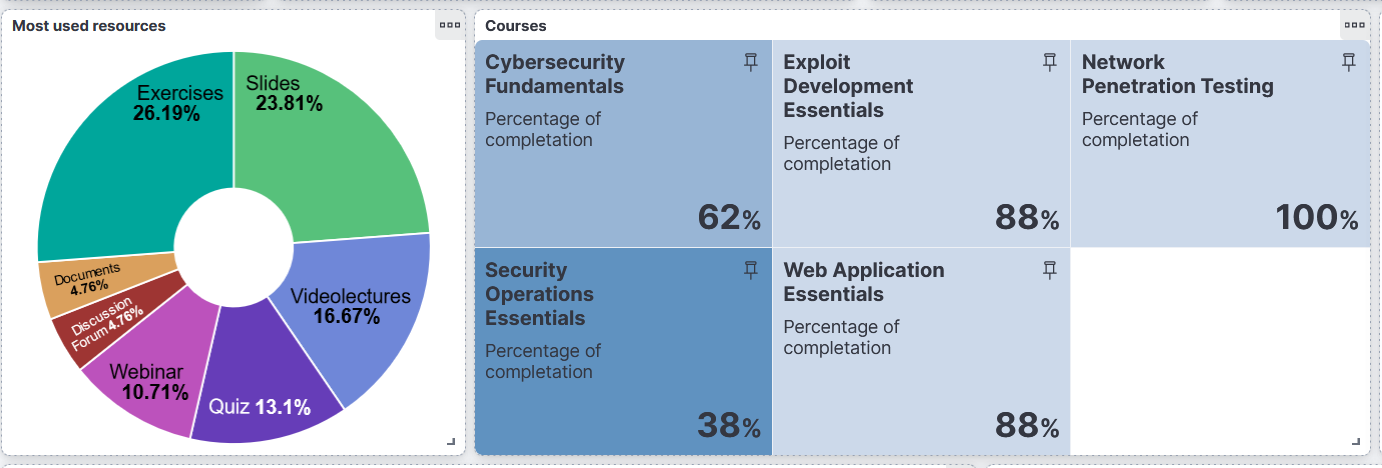
\includegraphics[width=0.9\textwidth]{assets/dashboard_1_122.png}
    \caption{Dashboard I - Subgoal 1.2.2}
    \label{fig:dashboard_1_subgoal_122}
\end{figure}

The four elements described above occupy the majority of the dashboard on 
the left side of the screen allowing the student to have a clear and complete
understanding of his/her engagement with the platform and how he/she has to
adapt his/her learning path, hence supporting the student's goals. 

The remaining part of the dashboard, following the
\textbf{Principle 4}, contains different elements that remind the student
situation regarding the subgoals of the first major goal (how he/she is upgrading 
his/her skill). 

\begin{figure}[H]
    \centering
    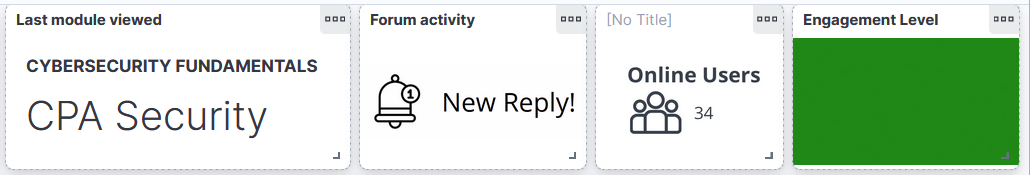
\includegraphics[width=0.9\textwidth]{assets/dashboard_1_globaltop.png}
    \caption{Dashboard I - Global Top}
    \label{fig:dashboard_1_global_top}
\end{figure}

These elements show student engagement with the platform by showing (from right to left)
the level of engagement computed with the CST described in a previous chapter,
how many students are online, a section
where are shown notifications from the forum 
and an element where is present the last viewed module helps the student
to remember what module was viewed last.
All these elements ensure to have the global situation awareness in each moment, 
to avoid the \textbf{Attentional Tunneling} demon. The student is not only focused
on his/her engagement with the platform or his/her state in the learning process but is
also aware of his/her results from all the tests he/she has done until now.

For this dashboard, the \textbf{Principle 1}, the \textbf{Principle 2} and the \textbf{Principle 3}
have been used as base principles to design the different elements. Thanks to that, the 
visualization of the student's goal is easy to find, since the elements are positioned in center-left
part of the screen. 

To support the student's comprehension and avoid the 
\textbf{Memory Trap} demon, the data are processed and integrated: the spider chart
(positioned on the right side) shows in a faster way the results of the student than
could be done with a table. For the same reason, the donut chart allows a clearer 
understanding of which resources the student prefers more. This kind of visualization of the
data helps in reducing the quantity of data to show in the dashboard to 
avoid the \textbf{Data Overload} demon. Consequently, the \textbf{Complexity Creep} demon is not present.

The \textbf{Principle 5} is supported by the element that communicates the number of 
notifications from the forum, which capture the attention of the student and
facilitate the change between goal-driven and data-driven processing. As said before
this element helps in avoiding the \textbf{Attentional Tunneling} demon.

The \textbf{Principle 6} is used to capture the student's attention on the course that
he/she has completed less. In addition to the percentage of completion of the course,
the intensity of the color of the element in the matrix decreases with the increase
of the percentage of completion, then guiding the student toward the course he/she has more to
do before the deadline of the courses. The engagement level element is displayed as a square
shape filled with a color (green, yellow, orange), it can capture the student's attention when is not needed, so 
causing a bit of the \textbf{Salience} demon. But this is not going to cause a
level of stress to reduce the working memory, as can be worse in other scenarios with 
faster dynamics.

In order to not get \textbf{Data Overload} demon, as said before, the data are visualized
more compactly, for example, is not shown the sequence of the votes of the student in
the home dashboard, but is shown a spider graph containing the results of the student on the
theory tests and the exercises tests, weighted on the number of tests completed for the course.

The \textbf{Out of the Loop} demon is not present inside the dashboard, because
the student is aware of his/her situation in the learning process, thanks to the results of each
test done until now, how many tests he/she has done. In addition, there is not any 
element that can work alone, without the intervention of the student, because in the 
learning process has to be the student to decide what to do and when to do it.

Regarding level three of
Situation Awareness, the linear graph helps the student to project the time he/she will
spend on the platform in the future on the base of the actual trend.


